\begin{minipage}{0.64\linewidth}
    Le solide $(S)$ de masse $m=\qty{200}{\gram}$ est fixé à un ressort
    horizontal à spires non jointives, de masse négligeable et de raideur $K$. À
    l'équilibre, le centre d'inertie $G$ de $(S)$ coïncide avec l'origine du
    repère ($O,\ex$) lié à la Terre supposé galiléen
    (figure~\ref{fig:solide_ressort}). Tous les frottements sont négligeables.
\end{minipage}
\hfill
\begin{minipage}{0.35\linewidth}
\begin{figure}[H]
    \centering
    \input{figures/solide_ressort.tex}
    \caption{}
    \label{fig:solide_ressort}
\end{figure}
\end{minipage}

On écarte ($S$) de sa position d'équilibre dans le sens positif d'une
distance $X_{m}$ et on l'abandonne sans vitesse initiale à $t_{0}=0$.

Le solide ($S$) effectue alors un mouvement de translation rectiligne
sinusoïdal de période propre $T_{0}$.
\begin{enumerate}
    \item Le solide ($S$) effectue 20 oscillations pendant la durée
          $\Delta t=\qty{12,6}{\second}$.

          Vérifier que $K=\qty{20}{\newton\per\meter}$.
\end{enumerate}
\begin{minipage}{0.64\linewidth}
    \begin{enumerate}
        \setcounter{enumi}{1}
        \item On choisit l'état où le ressort n'est pas déformé comme état de
              référence de l'énergie potentielle élastique $E_{pe}$ et le plan
              horizontal contenant $G$ comme état de référence de l'énergie
              potentielle de pesanteur $E_{pp}$.
    
              La courbe de la figure~(\ref{fig:Ec_de_t}) représente le diagramme
              d'énergie cinétique $E_{c}=f(t)$ du solide.
    
              En exploitant le diagramme, déterminer les valeurs de~:
              \begin{enumerate}
                  \item l'énergie mécanique $E_{m}$.
                  \item l'amplitude $X_{m}$.
                  \item l'abscisse $x_{1}$ du centre d'inertie $G$ de ($S$) à
                        l'instant $t_{1}=\qty{1,2}{\second}$.
              \end{enumerate}
    \end{enumerate}
\end{minipage}
\hfill
\begin{minipage}{0.35\linewidth}
 \begin{figure}[H]
    \centering
    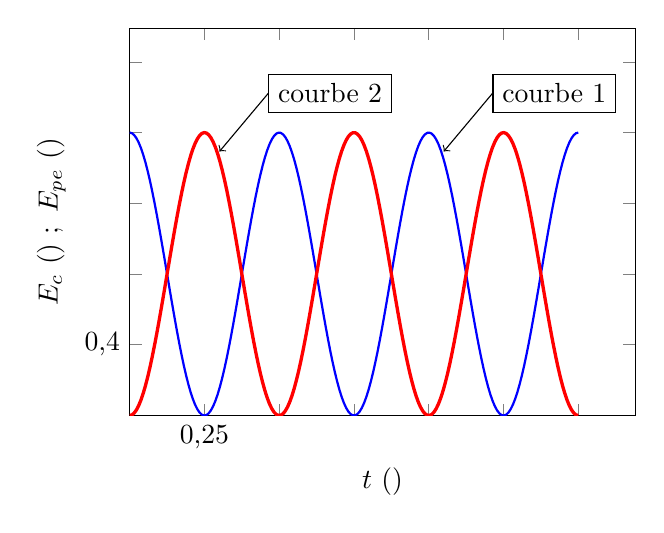
\begin{tikzpicture}
        \def\Xm{0.02}
        \def\T{1}
        \def\K{8}
        \pgfmathpi\let\pi=\pgfmathresult
        \begin{axis}[
                xmin=0,xmax=1.69,
                ymin=0,ymax=2.19,
                width=8cm,height=6.5cm,
                trig format plots=rad,
                xtick distance=0.25, ytick distance=0.4,
                xticklabels={,,{0,25}}, yticklabels={,,{0,4}},
                xlabel=$t~(\unit{\second})$,
                ylabel=$E_{c}~(\unit{\mJ})~;~E_{pe}~(\unit{\mJ})$,
            ]
            \addplot[domain=0:1.5,samples=200,thick,blue]
                {0.5*\K*\Xm*\Xm*cos(2*pi/\T*x)*cos(2*pi/\T*x)*1e3}
                coordinate[pos=0.68] (c1);
            \addplot[domain=0:1.5,samples=200,very thick,red]
                {0.5*\K*\Xm*\Xm*sin(2*pi/\T*x)*sin(2*pi/\T*x)*1e3}
                coordinate[pos=0.18] (c2);
        \end{axis}
        \draw[<-,shorten <=1pt] (c1) -- ++(50:1) node[right,draw] {courbe~1};
        \draw[<-,shorten <=1pt] (c2) -- ++(50:1) node[right,draw] {courbe~2};
    \end{tikzpicture}
    \caption{}
    \label{fig:Ec_de_t}
\end{figure}   
\end{minipage}

